% Figure: mean spaces of the ordered and unordered experiments (Section 3.1).
% One core mean (horizontal) and one redundant mean (vertical). With several inequalities in either
% group, the axes are the largest core mean and the largest redundant mean.
% Label 'excluded in both' added 2026-11-23 (R2-D2's wording).
% Colors (Federico's palette, 2026-11-23): null blue, alternative green, excluded in both experiments orange with hatching,
% excluded by the ordering only light gray with dots. Patterns keep the figure legible in grayscale. Luke, 2026-11-23. Compile with pdflatex.
\documentclass[border=1pt]{standalone}
\usepackage{amsmath,amssymb}
\usepackage{tikz}
\usetikzlibrary{patterns,arrows.meta}
\definecolor{nullc}{RGB}{214,226,243}
\definecolor{altc}{RGB}{218,235,224}
\definecolor{exclc}{RGB}{243,227,211}
\definecolor{ordc}{RGB}{236,236,236}
\definecolor{exclline}{RGB}{176,110,60}
\begin{document}
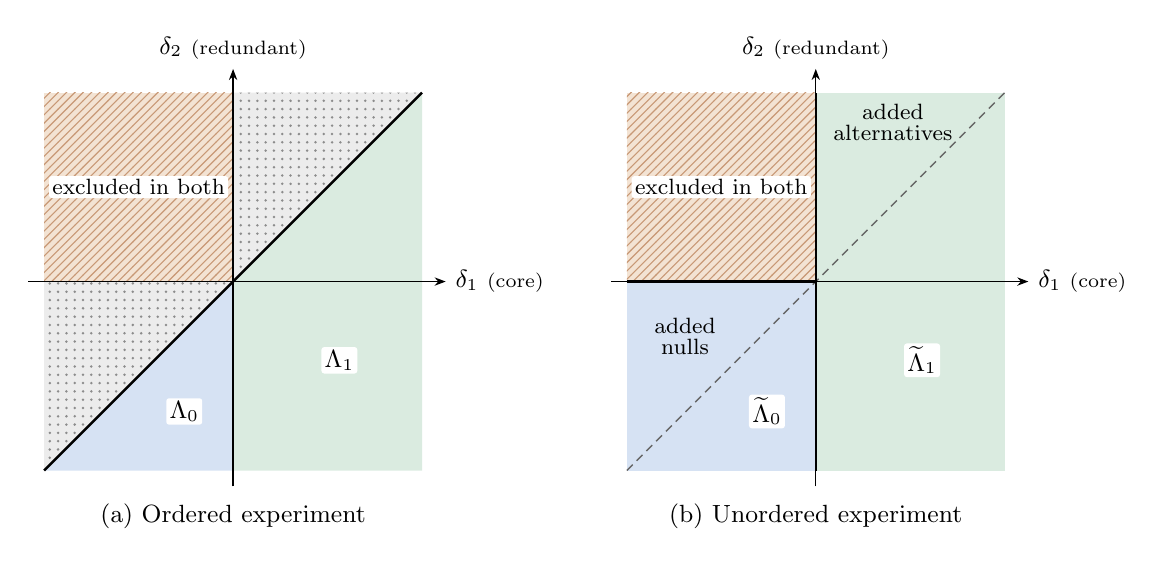
\begin{tikzpicture}[
  font=\small,
  null/.style={fill=nullc},
  alt/.style={fill=altc},
  common/.style={fill=exclc, postaction={pattern=north east lines, pattern color=exclline!70}},
  order/.style={fill=ordc, postaction={pattern=dots, pattern color=black!45}},
  ax/.style={-{Stealth[length=4pt]}, line width=0.5pt},
  bd/.style={line width=0.9pt},
  lab/.style={fill=white, inner sep=1.2pt, rounded corners=1pt},
]
\def\L{2.4}

% ---------------- (a) Ordered ----------------
\begin{scope}
  \fill[alt]  (0,0) -- (\L,\L) -- (\L,-\L) -- (0,-\L) -- cycle;
  \fill[null] (-\L,-\L) -- (0,0) -- (0,-\L) -- cycle;
  \fill[common] (-\L,0) rectangle (0,\L);
  \fill[order] (0,0) -- (0,\L) -- (\L,\L) -- cycle;
  \fill[order] (-\L,-\L) -- (0,0) -- (-\L,0) -- cycle;
  \draw[bd] (-\L,-\L) -- (\L,\L);
  \draw[bd] (0,0) -- (0,-\L);
  \draw[ax] (-\L-0.2,0) -- (\L+0.3,0) node[right] {$\delta_1$ \scriptsize(core)};
  \draw[ax] (0,-\L-0.2) -- (0,\L+0.3) node[above] {$\delta_2$ \scriptsize(redundant)};
  \node[lab] at (-0.62,-1.65) {$\Lambda_0$};
  \node[lab] at (1.35,-1.0) {$\Lambda_1$};
  \node[lab, font=\footnotesize] at (-1.2,1.2) {excluded in both};
  \node[below] at (0,-\L-0.3) {(a) Ordered experiment};
\end{scope}

% ---------------- (b) Modified ----------------
\begin{scope}[xshift=7.4cm]
  \fill[alt]  (0,-\L) rectangle (\L,\L);
  \fill[null] (-\L,-\L) rectangle (0,0);
  \fill[common] (-\L,0) rectangle (0,\L);
  \draw[densely dashed, line width=0.5pt, black!60] (-\L,-\L) -- (\L,\L);
  \draw[bd] (-\L,0) -- (0,0) -- (0,\L);
  \draw[bd] (0,0) -- (0,-\L);
  \draw[ax] (-\L-0.2,0) -- (\L+0.3,0) node[right] {$\delta_1$ \scriptsize(core)};
  \draw[ax] (0,-\L-0.2) -- (0,\L+0.3) node[above] {$\delta_2$ \scriptsize(redundant)};
  \node[lab] at (-0.62,-1.65) {$\widetilde\Lambda_0$};
  \node[lab] at (1.35,-1.0) {$\widetilde\Lambda_1$};
  \node[font=\footnotesize, align=center] at (0.98,2.02) {added\\[-2pt]alternatives};
  \node[font=\footnotesize, align=center] at (-1.66,-0.70) {added\\[-2pt]nulls};
  \node[lab, font=\footnotesize] at (-1.2,1.2) {excluded in both};
  \node[below] at (0,-\L-0.3) {(b) Unordered experiment};
\end{scope}
\end{tikzpicture}
\end{document}
